\chapter{ENSEMBLE APPROACH}
write about approach here

\subsection{Bayesian Combined Forecasting}
The BCF approach \cite{Petridis2001} is one of several types of methods which attempt to combine other forecasting models for time series. We selected this forecasting method over other multiple model forecasting methods (such as mixture of experts or ensembles of neural networks) due to its modularity and strong statistical backing.  BCF is modular in that it allows for the component forecasting models to come from any trained forecaster with a well defined distribution of the forecaster's mis-forecasts.  Its statistical backing comes from its direct derivation from Bayes' rule.

This section derives the BCF approach for readers unfamiliar with it and then describes some modifications of the approach which improves its performance for our application.

\subsection{Notation}
We define the time series dataset used in these models as $\{T_{t}^{(m)}\}$.  In our application the data used for these models comes from a set of $M$ binary infrared sensors.  Each $T_{t}^{m}$ is a 10 minute aggregate of the readings from sensor $m$ reading at time block $t$.  

Forecasts for a given model $k$ from the set of all models $K$ are represented by 
\begin{equation}
\bar{T}_{t + 1}^{k, m} = f(T_{t}, ..., T_{1}; \theta_{k}).
\end{equation}
\noindent
Thus the forecast of $T_{t + 1}$ is a function of all past data and some trained parameterization $\theta_{k}$ for that model. 

In this work we need to forecast more than one time step into the future.  Future forecasts are performed through iterative one step ahead forecasts.  Also for this work we forecast a model for each individual sensor and for convenience drop the $m$ from our forecasting notation.  An example of a forecast two time steps ahead of current time $t$ is given by 
\begin{equation}
\bar{T}_{t + 2}^{k} = f(\bar{T}_{t + 1}, T_{t}, ..., T_{1}; \theta_{k}).
\end{equation}
\noindent
Such a forecast is simply the forecast for one time step into the future but now with the forecasted value of $\bar{T}_{t + 1}$ used as the most recent datapoint to forecast $\bar{T}_{t + 2}$.  Forecasting in this nature allows for forecasts any number of time steps into the future. 

\begin{figure*}[t]
\centering
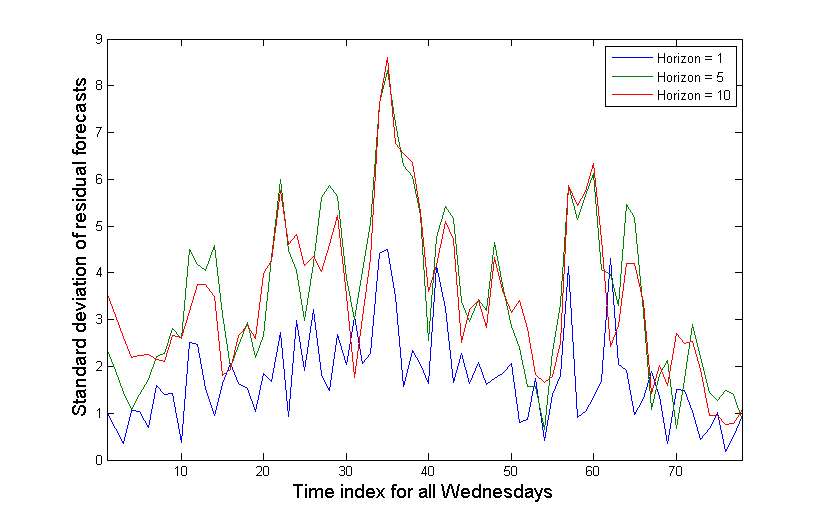
\includegraphics[width = .55\linewidth]{svm_standard_deviations_vs_horizon.png}
\caption{Standard deviation of support vector machine residuals for all Wednesdays in MERL dataset.  Time index represents 10 minute intervals from 6:00am to 7:00pm.}
\label{fig:svmstd}
\end{figure*}

\subsection{Bayesian Combined Forecasting Derivation}
To derive BCF we first assume the existence of $K$ models.  From these $K$ models, we want to create a probability distribution on a new random variable $z$ that is used to determine if model $k$ is the correct model from which to forecast at time $t$.  To do this we use the notation of Petridis \cite{Petridis2001} and define $p_{t}^{k}$ as follows
\begin{equation}
p_{t}^{k} = p(z = k | T_{t}, ..., T_{1}).
\end{equation}

From here we apply Bayes rule and get
\begin{equation}
p_{t}^{k} = \frac{p(T_{t} | z = k, T_{t - 1}, ..., T_{1}) \cdot p(z = k | T_{t - 1}, ..., T_{1})} {p(T_{t}, ..., T_{1})}.
\end{equation}
\noindent
Notice that $p(z = k | T_{t - 1}, ..., T_{1}) = p_{t - 1}^{k}$.  Thus we can create a recursive estimation based on prior $p_{t}^{k}$.

With recursive values for $p_{t}^{k}$ and replacing $p(T_{t}, ..., T_{1})$ with a conditional probability on $z$ we get
\begin{equation}
p_{t}^{k} = \frac{p(T_{t} | z = k, T_{t - 1}, ..., T_{1}) \cdot p_{t - 1}^{k}} {\sum_{j = 1}^{K}p(T_{t} | z = j, T_{t - 1}, ..., T_{1}) \cdot p_{t - 1}^{j}}.
\end{equation}

We use the empirically observed forecasting error for each model to estimate $p(T_{t}|z = k, T_{t - 1}, ..., T_{1})$.  The forecasting error for a given model at time $t$ is 
\begin{equation}
e_{t}^{k} = \bar{T}_{t}^{k} - T_{t}.
\end{equation}
\noindent
We can use these forecasting errors to estimate a probability distribution for each model on the random variable $e_{t}^{k}$.  This is typically modeled as a white noise zero mean Gaussian process.  For our work, we represent this as a distribution of error terms with some parameterization $\omega_{k}$.  Thus for each model the probability error distribution function on the model error random variable is given by $q(e_{t}^{k};\omega_{k})$.

The final equation for the posterior probability of a given model $k$ is
\begin{equation}
\label{eq:model_prob}
p_{t}^{k} = p(z = k|T_{t}, ..., T_{1}) = \frac{p_{t - 1}^{K} \cdot q(T_{t} - \bar{T}_{t}^{k}; \omega_{k})}{\sum_{j=1}^{K}p_{t - 1}^{j} \cdot q(T_{t}^{j} - \bar{T}_{t}^{j}; \omega_{j})}.
\end{equation}

An example of these changing normalized posterior probabilities for a small section of the MERL dataset is shown in Figure~\ref{fig:probsmerl}.

Forecasting using BCF is done by either computing a weighted forecast $\delta$ time steps into the future for each forecasting model or by simply selecting the model with the highest likelihood.  For this paper we forecast using a weighted forecast of all models.  The forecasting equation is
\begin{equation}
T_{t + \delta}^{ALL} = \sum_{k=1}^{K}p_{t}^{k} \cdot \bar{T}_{t + \delta}^{k}.
\end{equation}

\begin{figure}
\centering
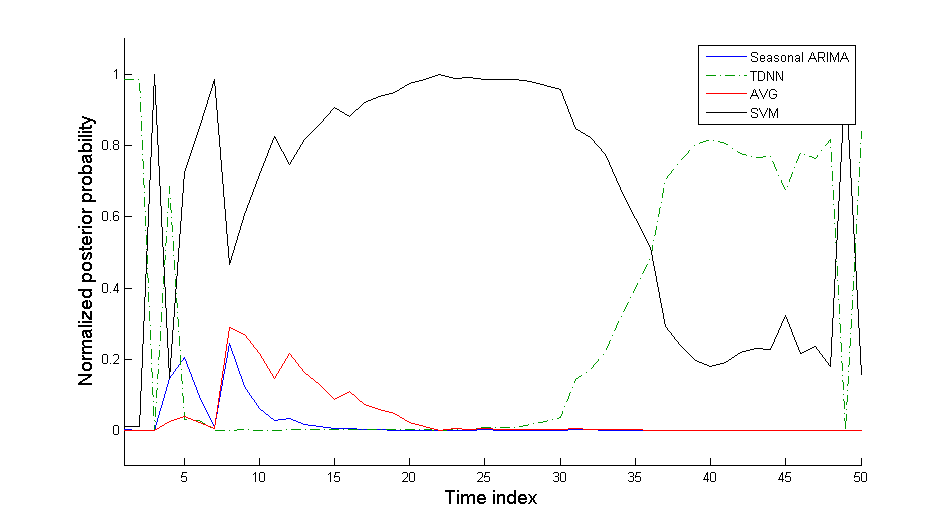
\includegraphics[width = 1.0\linewidth]{posterior_probs.png}
\caption{Normalized posterior probabilities of component models on a section of MERL dataset.}
\label{fig:probsmerl}
\end{figure}

\subsection{BCF Modifications}
In this subsection we discuss a number of modifications to maximize the effectiveness of BCF for our data.  We refer to the modified BCF algorithm as Bayesian Combined Forecasting for multiple Time Steps or BCF-TS for short.  These modifications  enable BCF to work with forecasting horizons greater than one in the future.

\subsubsection{Forecast $\delta$ time steps into the future}
Traditional implementations of BCF in other domains \cite{Petridis2001, Zheng2006} are interested only in 1 time step ahead forecasts.  For our work we require forecasts that are $\delta$ steps ahead which requires a small change to the BCF method.  Instead of generating a model's error distribution from 
\begin{equation}
e^{t}_{k} = \bar{T}_{t}^{k} - T_{t} = f(\bar{T}_{t},T_{t - 1} ..., T_{1}; \theta_{k}) - T_{t}.
\end{equation}

The error distribution is instead generated from 
\begin{equation}
e^{t}_{k} = f(\bar{T}_{t}, ..., \bar{T}_{t - \delta + 1}, T_{t - \delta}, ..., T_{1};\theta_{k}) - T_{t}.
\end{equation}
The reason for this change is due to the assumption that our error distribution is an accurate representation forecasting accuracy.  
The forecasting error distribution for models at $1$ time step into the future is not necessarily the same as models at $\delta$ time steps.  Thus we compute a different error distribution for each forecast time step.


\subsubsection{Improving model error distributions}
Despite other implementations of BCF using fixed error distributions, our data has clear daily trends.  For some of our models, the forecasted residuals follow these same trends.  See Figure~\ref{fig:svmstd} for an example of how the forecasting error distribution for a trained support vector regression model on the MERL dataset depends on the time and on the forecasting horizon.

To represent a more realistic error distribution instead of a fixed white noise Gaussian that is commonly used in the literature, we fit a Gaussian for each 10 minute slice of a given day.  The data from the MERL dataset was used from 6:00am to 7:00pm. The thirteen hours of data used per day represent 78 time slices.  For example taking the data for each time slice for each Wednesday results in 78 Gaussian error distributions for each forecasting horizon.  These Gaussians are computed from a validation set representing 20\% of our data.  It is from this set of models error distributions that we compute BCF.

As a possible improvement to this set of error distributions, we note that using a generalized autoregressive conditional heteroskedastic (GARCH) model \cite{Box2008} or some other appropriate model to forecast future variance based on local and historic changes in variance would likely outperform our time based average Gaussian models.  GARCH models are similar to seasonal autoregressive moving average models which we use as one of our component forecasting models.

\subsubsection{Model selection thresholding}
Diebold \cite{Diebold1991} cautions against the use of forecasting using a Bayesian combination of models in all cases.  Diebold points out that under certain situations a convex combination of forecasts for models may not be optimal, and cases exist where taking negative likelihood weighting may be optimal.  These conditions are likely to arise during instances where the data may not be accurately described by any of the forecasting models.  

Furthermore when such cases where no model is able to provide an accurate forecast, then it is often the case that forecasts come from the worst model.  

To combat this case, we have implemented a model selection threshold $h_{k}$.  If the likelihood of all component models is below $h_{k}$, then we forecast from only the model which is historically the most accurate based on our validation set.  

The threshold is different for each model, and should depend on the error distribution of the model.  In practice we have found that $2\sigma$ serves as a good threshold.  Basing the threshold on $\sigma$ is useful as it provides a threshold value which does not depend on $e^{k}_{t}$.  For a zero mean Gaussian the probability of the $2\sigma$ threshold is
\begin{equation}
p(2\sigma) = \frac{1}{\sigma\sqrt{2\pi}}e^{-2}.
\end{equation}
Because the Bayesian combined forecasting approach is iterative, it is possible that a long section of forecasts that indicate one model correct or incorrect can lead to likelihood underflow.  Due to this problem we adjust our normalized likelihoods so that no model may reach a value below 0.001.  This empirically chosen value is low enough to not have a great impact on forecasts while still being high enough to allow model likelihoods to change quickly.

\subsection{Results of Ensemble}

BCF and BCF-TS (BCF with our specific set of modifications) were trained and tested using all component models described above.  All of the models were trained on 60\% of the total datasets.  Another 20\% was used for model validation and the final 20\% used for testing.  All results shown below are on the test set only.  Figure~\ref{fig:realbcf} shows an sample section of test data from the MERL dataset along with BCF-TS forecasts for horizons of 1 and 5.   As expected as the forecasting horizon increases the forecasts become less accurate.

\begin{figure}[h]
\centering
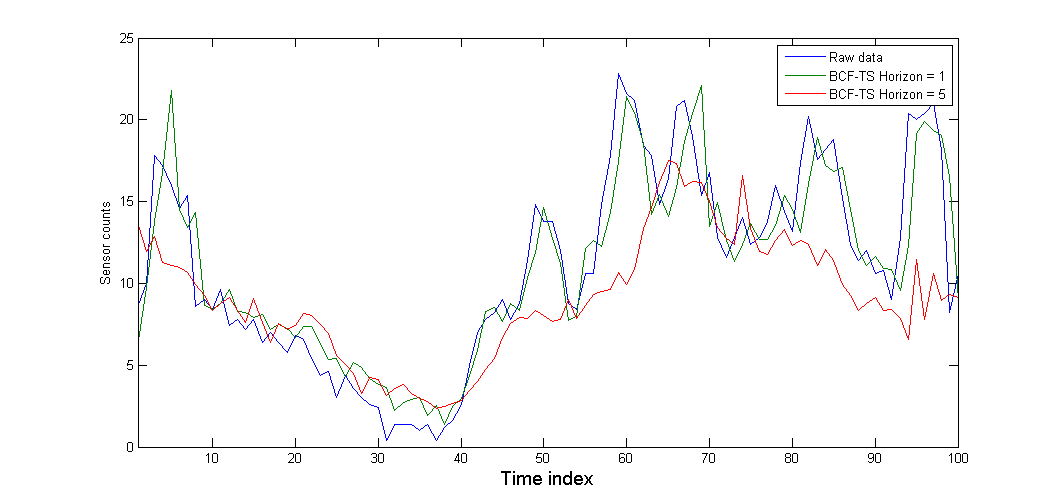
\includegraphics[width = 1.0\linewidth]{real_forecasts_bcf.png}
\caption{A comparison of forecasts at various horizons against real data for an sample time segment using BCF-TS.}
\label{fig:realbcf}
\end{figure}

It is common for one model's normalized posterior probability to be near one when that model is currently accurate.  Figure~\ref{fig:realbcfsvm} shows as example of this behavior.  From time index 1 to 8, the SVM component model has a posterior probability near 1.0 and as a result BCF-TS forecasts nearly completely from this model.  Then from time index 9 on the model's posterior probability is lower and as a result BCF-TS uses other model for its combined forecast.

\begin{figure}[h]
\centering
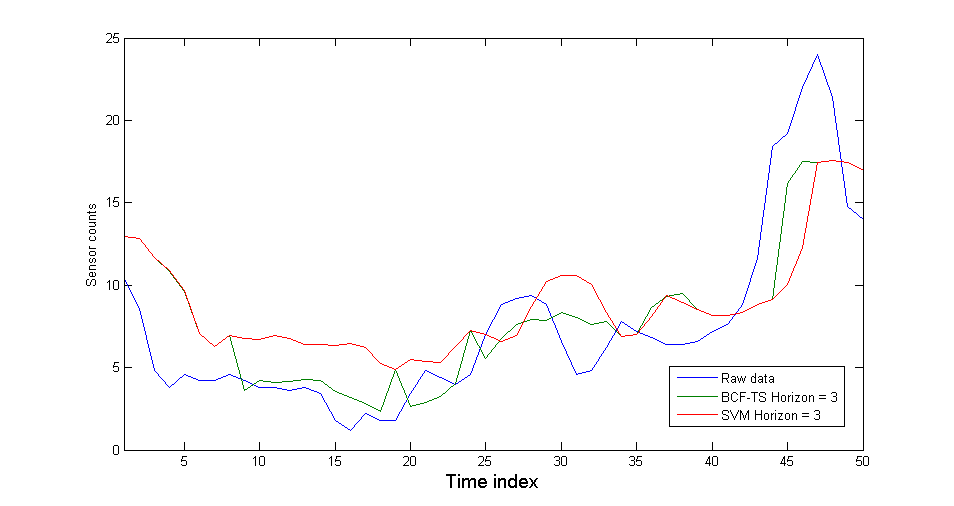
\includegraphics[width = 1.0\linewidth]{real_forecasts_bcf_svm.png}
\caption{A comparison of BCF-TS and SVM forecasts at horizon equal to three against real data.}
\label{fig:realbcfsvm}
\end{figure}

Figure~\ref{fig:rmseplot} shows the results of the root mean squared error (RMSE) of forecasts across a forecast horizon up to 10 time steps (100 minutes) into the future for each model.  These plots show that BCF-TS has the lowest error.  However, the average model shows itself to be a strong indicator of future activity for forecasts beyond 60 minutes into the future.  Forecasts were performed for significantly longer horizons, but the results were uninteresting as the total RMSE of models converged to roughly the values at a forecasting horizon of 10 time steps.  

\begin{table}
\centering
\caption{Run times (in seconds) for each forecasting horizon.}
\begin{tabular}{|c|c|c|c|c|c|c|c|} \hline
Algorithm & $1$ & $2$ & $3$ & $5$ & $8$ & $10$ \\ \hline
Average & 0.001 & 0.001 & 0.001 & 0.001 & 0.001 & 0.001 \\ \hline
ARIMA & 0.043 & 0.045 & 0.046 & 0.053 & 0.058 & 0.063\\ \hline
SVM & 0.048 & 0.910 & 0.137 & 0.227 & 0.357 & 0.444 \\ \hline
TDNN & 20.87 & 21.60 & 21.82 & 21.28 & 22.73 & 22.50 \\ \hline
BCF-TS & 20.97 & 21.26 & 21.27 & 21.34 & 21.57 & 21.63\\ \hline
\end{tabular}
\label{fig:runtimestab}
\end{table}

In the CSMBB dataset the Seasonal ARIMA model was a good forecaster of future activity while in the MERL set it performed significantly worse than even the average model on all forecasting horizons.  This is likely due to a stronger seasonal component to the CSMBB dataset due class schedules.  Instead on the MERL dataset there is little seasonal correlation and thus natural variance from a prior season may incorrectly affect current forecasts.  This result is similar to that of other papers that use seasonal ARIMA models \cite{Newsham2010}; where in the case of strong seasonal data, results are better for short horizon forecasts, but longer forecasts favor historic averages.

BCF and BCF-TS were both better at a horizon of one time step for all component models (see Table~\ref{fig:rmsetab}).  In the MERL dataset standard BCF was outperformed by SVM and later the average model for all forecast beyond one horizon.  However the BCF-TS model showed significant improvement in RMSE scores for all forecasting horizons unto 60 minutes.  For horizons of 10 time steps and greater, the average model is about as good as the BCF-TS approach.

Table~\ref{fig:runtimestab} shows the run time in seconds of each forecasting algorithm at a given forecasting horizon.  The times are for forecasting the entire test set on the MERL dataset for a single sensor, approximately twenty weeks worth of data.  In general BCF-TS was slower than any component model, but the times are still such that real-time forecasting is possible.

\begin{figure}[!ht]
	\begin{center}
		\subfigure[] {
			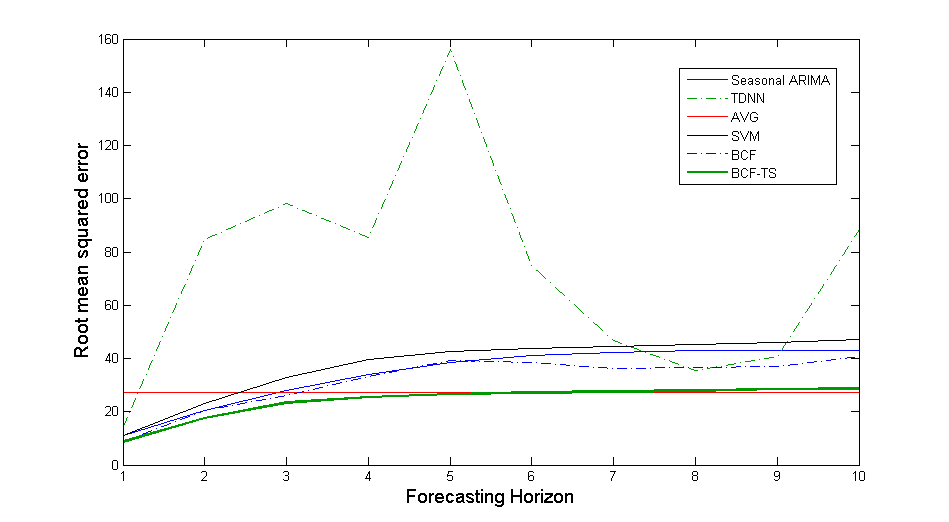
\includegraphics[width=0.49\linewidth]{brown_rmse.png}
			%\caption{CSMBB forecasting model errors}
			%\label{fig:csmrmse}
		}
		\subfigure[] {
			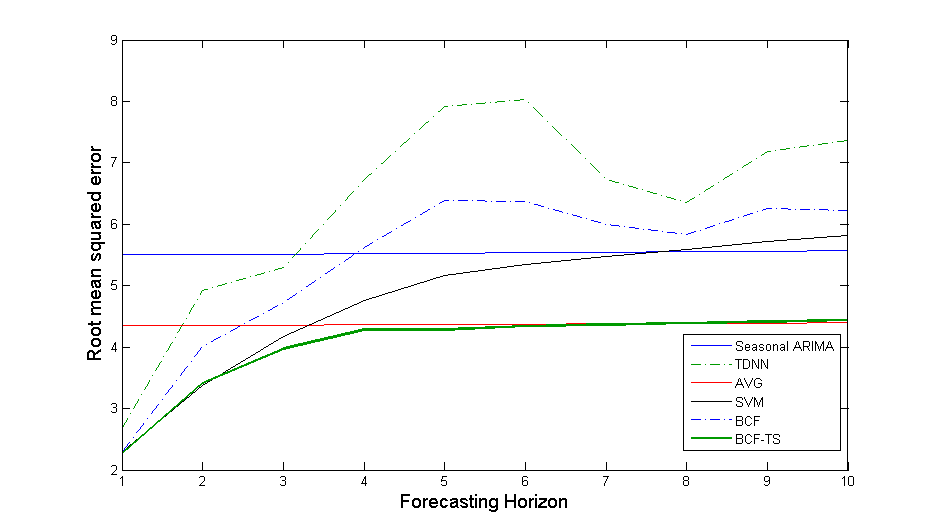
\includegraphics[width=0.49\linewidth]{merl_rmse.png}
			%\caption{MERL forecasting model errors}
			%\label{fig:merlrmse}
		}
	\end{center}
	\caption{Root mean square error of forecasting for each model vs forecasting horizon.}
	\label{fig:rmseplot}
\end{figure}


